\documentclass[12pt,a4paper,oneside]{article}

\usepackage[utf8]{inputenc}
\usepackage[portuguese]{babel}
\usepackage[T1]{fontenc}
\usepackage{amsmath}
\usepackage{amsfonts}
\usepackage{amssymb}
\usepackage{graphicx}

\usepackage{xcolor}
% Definindo novas cores
\definecolor{verde}{rgb}{0.25,0.5,0.35}
\definecolor{jpurple}{rgb}{0.5,0,0.35}
% Configurando layout para mostrar codigos Java
\usepackage{listings}
\lstset{
  language=Java,
  basicstyle=\ttfamily\small, 
  keywordstyle=\color{jpurple}\bfseries,
  stringstyle=\color{red},
  commentstyle=\color{verde},
  morecomment=[s][\color{blue}]{/**}{*/},
  extendedchars=true, 
  showspaces=false, 
  showstringspaces=false, 
  numbers=left,
  numberstyle=\tiny,
  breaklines=true, 
  backgroundcolor=\color{cyan!10}, 
  breakautoindent=true, 
  captionpos=b,
  xleftmargin=0pt,
  tabsize=4
}

\author{\\Universidade Federal de Goiás (UFG) - Regional Jataí\\Bacharelado em Ciência da Computação \\Teoria de Grafos \\Esdras Lins Bispo Jr.}

\title{\sc \huge Quarto Teste}

\date{22 de agosto de 2017}

\begin{document}

\maketitle

{\bf ORIENTAÇÕES PARA A RESOLUÇÃO}

\footnotesize

\begin{itemize}
	\item A avaliação é individual, sem consulta;
	\item A pontuação máxima desta avaliação é 10,0 (dez) pontos, sendo uma das 06 (seis) componentes que formarão a média final da disciplina: quatro testes, uma prova e os exercícios de aquecimento;
	\item A média final ($MF$) será calculada assim como se segue
	\begin{eqnarray}
		MF & = & MIN(10, S) \nonumber \\
		S & = & (\sum_{i=1}^{4} 0,2.T_i ) + 0,2.P  + 0,1.EA \nonumber
	\end{eqnarray}
	em que 
	\begin{itemize}
		\item $S$ é o somatório da pontuação de todas as avaliações,
		\item $T_i$ é a pontuação obtida no teste $i$,
		\item $P$ é a pontuação obtida na prova, e
		\item $EA$ é a pontuação total dos exercícios de aquecimento.
	\end{itemize}
	\item O conteúdo exigido compreende os seguintes pontos apresentados no Plano de Ensino da disciplina: (5) Cortes e Pontes, (6) Árvores, (7) Isomorfismo e (9) Planaridade.
\end{itemize}


\begin{center}
	\fbox{\large Nome: \hspace{10cm}}
\end{center}

\newpage

\normalsize

\begin{enumerate}

	\item (5,0 pt) {\bf [E 2.7]} Os grafos abaixo são isomorfos? Justifique.
	\begin{center}
		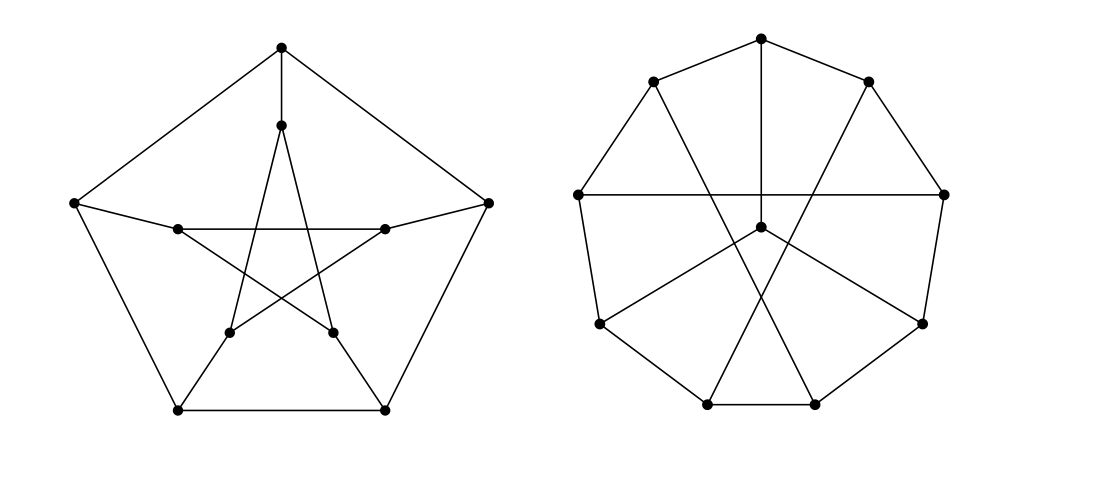
\includegraphics[width=\textwidth]{images/grafos.png}
	\end{center} 
	
	{ \color{blue} {\bf Resposta:} 
		
		Sim, são isomorfos. Seja a rotulação dos vértices dos dois grafos conforme se segue:
		\begin{center}
			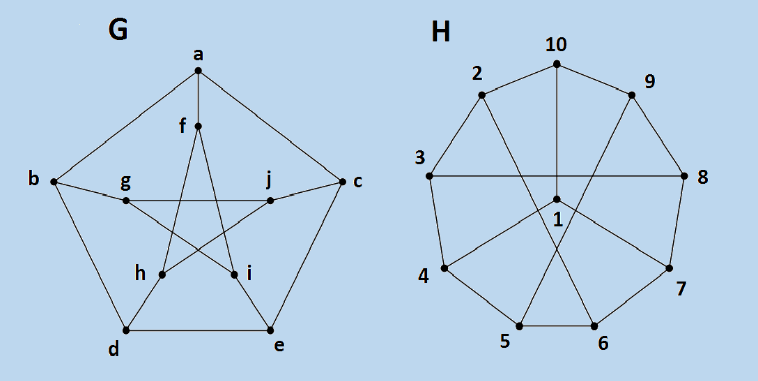
\includegraphics[width=0.8\textwidth]{images/grafos-rotulados.png}
		\end{center}
		É possível estabelecer uma bijeção entre $V_G$ e $V_H$ de forma a preservar as relações de adjacências entre os grafos. A bijeção é dada a seguir:
		\begin{center}
			\begin{tabular}{c|cccccccccc}
				$V_G$ 	&	a 	& b & c & d & e & f & g & h & i & j \\
				\hline
				$V_H$ 	&	10 	& 2 & 9 & 3 & 8 & 1 & 6 & 4 & 7 & 5 \\
			\end{tabular}
		\end{center}
		Como foi possível estabelecer a bijeção, os dois grafos são isomorfos $\blacksquare$
	}
	
	\item (5,0 pt) Na linguagem C, complete as lacunas da função {\tt contemCircuito} conforme apresentada abaixo. Você deve substituir apenas as linhas 6 e 9, pelos trechos de código 1 e 2, respectivamente. O objetivo é que esta função retorne valor 1, se o grafo fornecido como parâmetro contiver um circuito. O valor de retorno será 0, caso não for.

\begin{lstlisting}[language=C]
int contemCircuito(Grafo *g){

	for(int v=0; v<g->n; v++)
		for(int w=0; w<g->n; w++)
			if( g->adj[v][w] == 1){
				// TRECHO 1
			}
			
	//TRECHO 2
	
}\end{lstlisting}

{\color{blue} \bf Resposta: } \\
\begin{lstlisting}[language=C]
//TRECHO 1
if(ehPonte(g, v, w) == 0)
	return 1;
\end{lstlisting}

\begin{lstlisting}[language=C]
//TRECHO 2
return 0;
\end{lstlisting}
	
\end{enumerate}

\newpage

\section{grafos.h}

\begin{lstlisting}[language=C]
#ifndef GRAFO_H_INCLUDED
#define GRAFO_H_INCLUDED

#include <stdlib.h>

typedef struct grafo {
	char *nome;
	int n;       // Numero de vertices
	int m;       // Numero de arestas
	int **adj;   // Ponteiro para a matriz de adjacencias
} Grafo;

int **gerarMatriz(int n);
void inicializar(Grafo *g, char *nome, int n);
void inserirAresta(Grafo *g, int v, int w);
void removerAresta(Grafo *g, int v, int w);
void exibir(Grafo *g);
int grau(Grafo *g, int v);
int grauMinimo(Grafo *g);
int grauMaximo(Grafo *g);
int ehRegular(Grafo *g);
int eh3Regular(Grafo *g);
Grafo *gMenosV(Grafo *g, int v);
int ehCaminho(Grafo *g);
int ehConexo(Grafo *g);
int ehPonte(Grafo *g, int v, int w);

#endif // GRAFO_H_INCLUDED\end{lstlisting}

\newpage

\section{fabrica.h}

\begin{lstlisting}[language=C]
#ifndef FABRICA_H_INCLUDED
#define FABRICA_H_INCLUDED

#include <stdlib.h>
#include "grafo.h"

Grafo *k(int n);
Grafo *caminho(int n);
Grafo *circuito(int n);

#endif // FABRICA_H_INCLUDED\end{lstlisting}

\end{document}